\documentclass{beamer}
\usetheme{metropolis}
\usepackage{graphicx}
\usepackage{subfig}
\usepackage{tcolorbox}
\title{Algebra-Based Physics-2: Electricity, Magnetism, and Modern Physics (PHYS135B-01): Unit 1}
\author{Jordan Hanson}
\institute{Whittier College Department of Physics and Astronomy}

\begin{document}
\maketitle

\section{Unit 0 Review}

\begin{frame}{Unit 0 Review}
\textit{Physics} - $\phi\upsilon\sigma\iota\kappa\acute{\eta}$ - "phusik\'e": \textit{knowledge of nature} \\
from $\phi\acute{\upsilon}\sigma\iota\varsigma$ - "ph\'usis": \textit{nature} \\
\textbf{Reading: Chapters 18 and 19 (for Unit 1)}
\begin{enumerate}
\item Estimation/Approximation
\begin{itemize}
\item \alert{Estimating} the correct order of magnitude
\item \alert{Building} complex quantities
\item \alert{Unit analysis}
\end{itemize}
\item Review of concepts from Newtonian mechanics
\begin{itemize}
\item Kinematics and \alert{Newton's Laws}
\item Work-energy theorem, energy conservation
\item Momentum, conservation of momentum
\end{itemize}
\end{enumerate}
\end{frame}

\section{Unit 0 Review Problems}

\section{Summary}

\begin{frame}{Welcome to Electromagnetism and Modern Physics!}
\centering
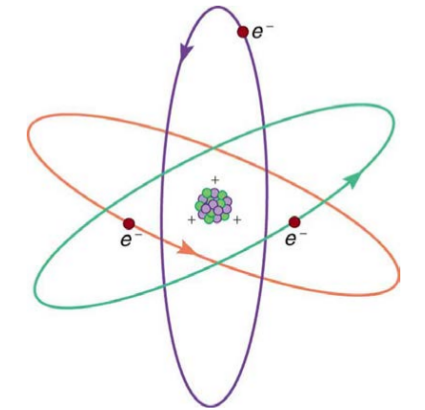
\includegraphics[width=0.7\textwidth]{figures/orbital.png}
\end{frame}

\begin{frame}{Welcome to Electromagnetism and Modern Physics!}
\centering

\includegraphics[width=0.7\textwidth]{figures/manhattan.jpg}
\end{frame}

\begin{frame}{Welcome to Electromagnetism and Modern Physics!}
\centering

\includegraphics[width=0.7\textwidth]{figures/manhattan2.jpg}
\end{frame}

\begin{frame}{Unit 1 Summary}
\textbf{Reading: Chapters 18 and 19}
\begin{enumerate}
\item Charge, mass, the Coulomb force, and the gravitational force
\item Force fields
\item Electric potential and capacitance
\end{enumerate}
\end{frame}

\section{JITT - Reading Quiz Results}

\section{Charge, Conductors and Insulators}

\begin{frame}{Charge, Conductors and Insulators}
Let's begin this topic in a special way: comparison to \textit{gravity}.  What do electricity and gravity have in common?  The answer lies in a notion we call \textit{charge...}
\end{frame}

\begin{frame}{Charge, Conductors and Insulators}
\centering
\textbf{\alert{Charge: the constant of proportionality between the strength of a \textit{field} and the force a field exerts on an \textit{object}.}} \\
\hrulefill
\small
\begin{columns}[T]
\begin{column}{0.5\textwidth}
\alert{Gravity}
\begin{enumerate}
\item Force: $\vec{F} = G \frac{m M}{r^2} \hat{r}$
\item Parameters: $r$ is absolute distance between two objects with masses $m$ and $M$, and the direction is $\hat{r}$
\item \textit{Charge} of one object: $m$
\item \textit{Field felt by that object}: $\vec{G} = G \frac{M}{r^2} \hat{r}$
\item $\vec{F} = m \vec{G}$
\end{enumerate}
\end{column}
\begin{column}{0.5\textwidth}
\alert{Electricity}
\begin{enumerate}
\item Force: $\vec{F} = k \frac{q Q}{r^2} \hat{r}$
\item Parameters: $r$ is absolute distance between two objects with electric charges $q$ and $Q$, and the direction is $\hat{r}$
\item \textit{Charge} of one object: $q$
\item \textit{Field felt by that object}: $\vec{E} = G \frac{Q}{r^2} \hat{r}$
\item $\vec{F} = q \vec{E}$
\end{enumerate}
\end{column}
\end{columns}
\end{frame}

\begin{frame}{Charge, Conductors and Insulators}
\centering
\textbf{\alert{Charge: the constant of proportionality between the strength of a \textit{field} and the force a field exerts on an \textit{object}.}} \\
\hrulefill \\
\small
In the field paradigm, objects with charges \textit{emanate} fields, causing other objects with charge to experience force. \\
\hrulefill \\
\begin{columns}[T]
\begin{column}{0.5\textwidth}
\alert{Gravity} \\
How many \textit{types of charge}, or how many charges, exist under the force of gravity? \\
\textbf{One.} We call it mass.
\end{column}
\begin{column}{0.5\textwidth}
\alert{Electricity} \\
How many \textit{types of charge}, or how many charges, exist under the force of electricity? \\
\textbf{Two.} We call one positive, and one negative.
\end{column}
\end{columns}
\end{frame}

\begin{frame}{Charge, Conductors and Insulators}
\centering
\textbf{\alert{Charge: the constant of proportionality between the strength of a \textit{field} and the force a field exerts on an \textit{object}.}} \\
\hrulefill \\
\small
In the field paradigm, objects with charges \textit{emanate} fields, causing other objects with charge to experience force. \\
\hrulefill \\
In the field paradigm, gravity has one charge (mass), and electricity has two charges (positive and negative). \\
\hrulefill \\
\textbf{There is one fundamental fact that is puzzling.} What about Newton's 2nd law?  Acceleration is not a field, it is a kinematic function.
\begin{equation}
\vec{F}_{\rm net} = m \vec{a}
\end{equation}
Aparently there are \textit{two kinds of mass}: \textbf{inertial} and \textbf{gravitational}.  
\end{frame}

\begin{frame}{Charge, Conductors and Insulators}
\small
\textit{Equivalence principle:} \\ \hrulefill \\
There are \textit{two kinds of mass}: \textbf{inertial} and \textbf{gravitational}, with \textbf{equal value} for a given object. \\ \vspace{0.5cm}
\url{https://en.wikipedia.org/wiki/Equivalence_principle} \\
\hrulefill \\
There is no similar principle for charge.  If the electric force on a charged object is calculated, that force must still be inserted into \textbf{Newton's 2nd Law} to obtain the acceleration, and the inertial mass must be known.
\end{frame}

\begin{frame}{Charge, Conductors and Insulators}
\small
Charge has other properties, some similar to gravitational mass: \\ \vspace{0.25cm}
\begin{enumerate}
\item Charge is conserved globally (charge cannot be created nor destroyed).  Mass has the same property.
\item Charge is conserved locally (if we pull charge out of the system, charge will flow into the system).
\item Charge is quantized, with an electron (for example) having the fundamental negative unit, and a proton (for example) having the fundamental positive unit.
\item The laws of physics are the same for positive and negative charges.
\item The two kinds of charge emit fields that attract each other; fields emitted by charges of the same type repel such charges.
\end{enumerate}
\end{frame}

\begin{frame}{Charge, Conductors and Insulators}
\textbf{Benjamin Franklin and the Leyden Jar}.  (Good paper topic).
\begin{figure}
\centering
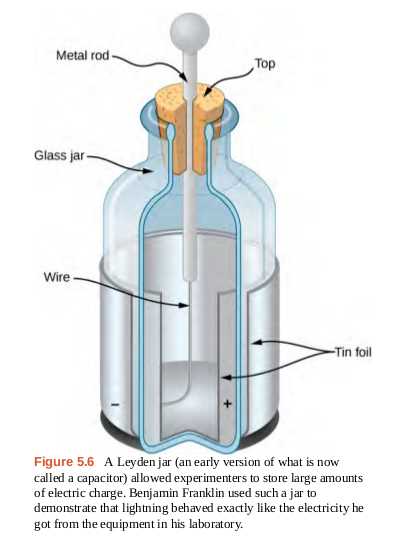
\includegraphics[width=0.3\textwidth]{figures/leyden.png}
\caption{\label{fig:leyden} A Leyden jar was an early version of a capacitor.  Benjamin Franklin guessed that one type of charge moves and another remains stationary, explaining several behaviors of charged objects.}
\end{figure}
\end{frame}

\begin{frame}{Charge, Conductors and Insulators}
The rest of the properties of charge are connected to the development of the structure of the atom, and we will return to this topic at the end of the semeter.
\begin{figure}
\centering
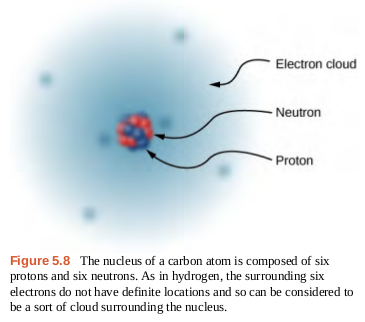
\includegraphics[width=0.5\textwidth]{figures/atom.png}
\caption{\label{fig:atom} A sketch of our current atomic paradigm.}
\end{figure}
\end{frame}

\begin{frame}{Charge, Conductors and Insulators}
Suppose an ion is composed of six protons, eight neutrons, and five electrons.  What is the net charge?
\begin{itemize}
\item A: +1
\item B: 0
\item C: -1
\item D: -2
\end{itemize}
\end{frame}

\begin{frame}{Charge, Conductors and Insulators}
A rod with a positive charge is held next to a \textit{conductor} (an object were charge can move around freely).  Which of the following is true?
\begin{itemize}
\item A: The charges in the conductor all remain in place because charge is conserved.
\item B: The negative charges in the conductor move toward the positive charges in the rod.
\item C: The positive charges remain in place but the negative charges move away from the rod.
\item D: The positive charges move toward the rod and the negative charges remain in place.
\end{itemize}
\end{frame}

\section{Coulomb’s Law and Electric Fields}

\begin{frame}{Coulomb’s Law and Electric Fields}
\textbf{Coulomb's Law} describes the force between charges. \\ \vspace{0.5cm}
\begin{tcolorbox}[colback=white,colframe=red!40!blue,title=Coulomb's Law]
\alert{The electric force, or \textbf{Coulomb force}, between two electrically charged systems with charges $q_{\rm 1}$ and $q_{\rm 2}$ separated by a distance $r$ is
\begin{equation}
\vec{F}_{\rm C} = \frac{1}{4\pi\epsilon_{\rm 0}} \frac{q_{\rm 1} q_{\rm 2}}{r^2} \hat{r} \label{eq:C}
\end{equation}
In Eq. \ref{eq:C}, $\hat{r} = \vec{r}/|\vec{r}|$, and $\epsilon_{\rm 0} = 8.85418782\times 10^{-12} N^{-1} m^{-2} C^2$, called the \textit{perimittivity of free space.}}
\end{tcolorbox}
\end{frame}

\begin{frame}{Coulomb’s Law and Electric Fields}
\begin{tcolorbox}[colback=white,colframe=red!40!blue,title=Coulomb Field]
\alert{The electric field corresponding to Eq. \ref{eq:C}, experienced by a charge $q$ and generated by a charge $Q$ is 
\begin{equation}
\vec{E}_{\rm C} = \frac{1}{4\pi\epsilon_{\rm 0}} \frac{Q}{r^2} \hat{r} \label{eq:Cf}
\end{equation}
In Eq. \ref{eq:Cf}, $r$ remains the separation between $q$ and $Q$.}
\end{tcolorbox}
Thus we have: $\vec{F}_{\rm C} = q \vec{E}_{\rm C}$. \\ \vspace{0.5cm}
The SI Unit of charge is the Coulomb, which is equal to the amount of charge in a "current" of 1 amp for 1 second (more on this later).  \textbf{The charge of an electron is $1.6\times 10^{-19}$ Coulombs, or C.}
\end{frame}

\begin{frame}{Coulomb’s Law and Electric Fields}
Have you noticed that the Coulomb force does not depend on kinematic variables like velocity, or have any dissipative effect?  Perhaps it is \alert{\textbf{conservative}}.  In your own words at your table, discuss the meaning of a conservative force. \\ \vspace{0.5cm}
\small
If a force $F$ is conservative, what is the relationship between $F$ and the potential energy, $U$?
\begin{itemize}
\item A: $F$ is proportional to the kinetic energy, which is related to $U$.
\item B: $F$ is proportional to the change in $-U$
\item C: Work done on a system going against $F$ is path independent, so $U$ is the same if the system's path is closed
\item D: B and C
\end{itemize}
\end{frame}

\begin{frame}{Coulomb’s Law and Electric Fields}
If a force is conservative, it is true that
\begin{equation}
F = -\frac{\Delta U}{\Delta x}
\end{equation}
In kinematics, $U$ is the potential energy.  In electrostatics, we write it as a \textit{voltage.}
\begin{equation}
E = -\frac{\Delta V}{\Delta x}
\end{equation}
\end{frame}

\begin{frame}{Coulomb’s Law and Electric Fields}
Suppose a charge $+q$ experiences the Coulomb field of another charge of $-2q$, separated by a distance $r$.  Which of the following is true?
\begin{itemize}
\item A: The charge $+q$ accelerates towards the other charge, and the charge $-2q$ remains stationary, because opposite charges attract.
\item B: The charge $-2q$ accelerates towards the other charge, and the charge $+q$ remains stationary, because opposite charges attract.
\item C: No charges move; the force on one is equal to the force on the other.
\item D: The charges accelerate towards each other.
\end{itemize}
\end{frame}

\begin{frame}{Coulomb’s Law and Electric Fields}
The answer to the previous problem involves Newton's Third Law.
\begin{figure}
\centering
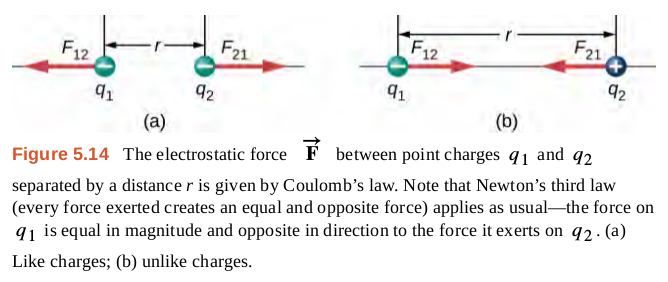
\includegraphics[width=0.9\textwidth]{figures/third.png}
\caption{\label{fig:third} Newton's Third Law still applies.}
\end{figure}
\end{frame}

\begin{frame}{Coulomb’s Law and Electric Fields}
Suppose a charge $+q$ experiences the Coulomb fields of two other charges of $-2q$, each located a distance $r$ from $+q$.  The charges are all colinear (on the same line).  Which of the following is true?
\begin{itemize}
\item A: The charge $+q$ accelerates towards one of the other charge, because opposite charges attract.
\item B: The charges $-2q$ accelerate towards the charge $+q$.
\item C: The charges $-2q$ accelerate towards the charge $+q$, but eventually repel each other back in the other direction.
\item D: The charges $-2q$ repel each other from the start.
\end{itemize}
\end{frame}

\begin{frame}{Coulomb’s Law and Electric Fields}
\small
The Coulomb force equation gives a vector, and so does the corresponding electric field.  Like a gravitational field, this effect has a vector at each point in space, so we refer to the Coulomb force and the Coulomb field as \textit{vector fields}. \\ \vspace{0.5cm}
\textbf{Vector field}: An assignment of a vector to each point in a subset of space.
\end{frame}

\begin{frame}{Coulomb’s Law and Electric Fields}
\small
\begin{columns}[T]
\begin{column}{0.5\textwidth}
Which of the following is true of vectors $\vec{v}_{\rm i}$ in the lower left-hand corner of the figure at right?
\begin{itemize}
\item A: They are probably $\vec{v}_{\rm i} = -\hat{i}-\hat{j}$
\item B: They are probably $\vec{v}_{\rm i} = \hat{i}+\hat{j}$
\item C: They are probably $\vec{v}_{\rm i} = -\hat{i}+\hat{j}$
\item D: They are probably $\vec{v}_{\rm i} = \hat{i}-\hat{j}$
\end{itemize}
\end{column}
\begin{column}{0.5\textwidth}
\begin{figure}
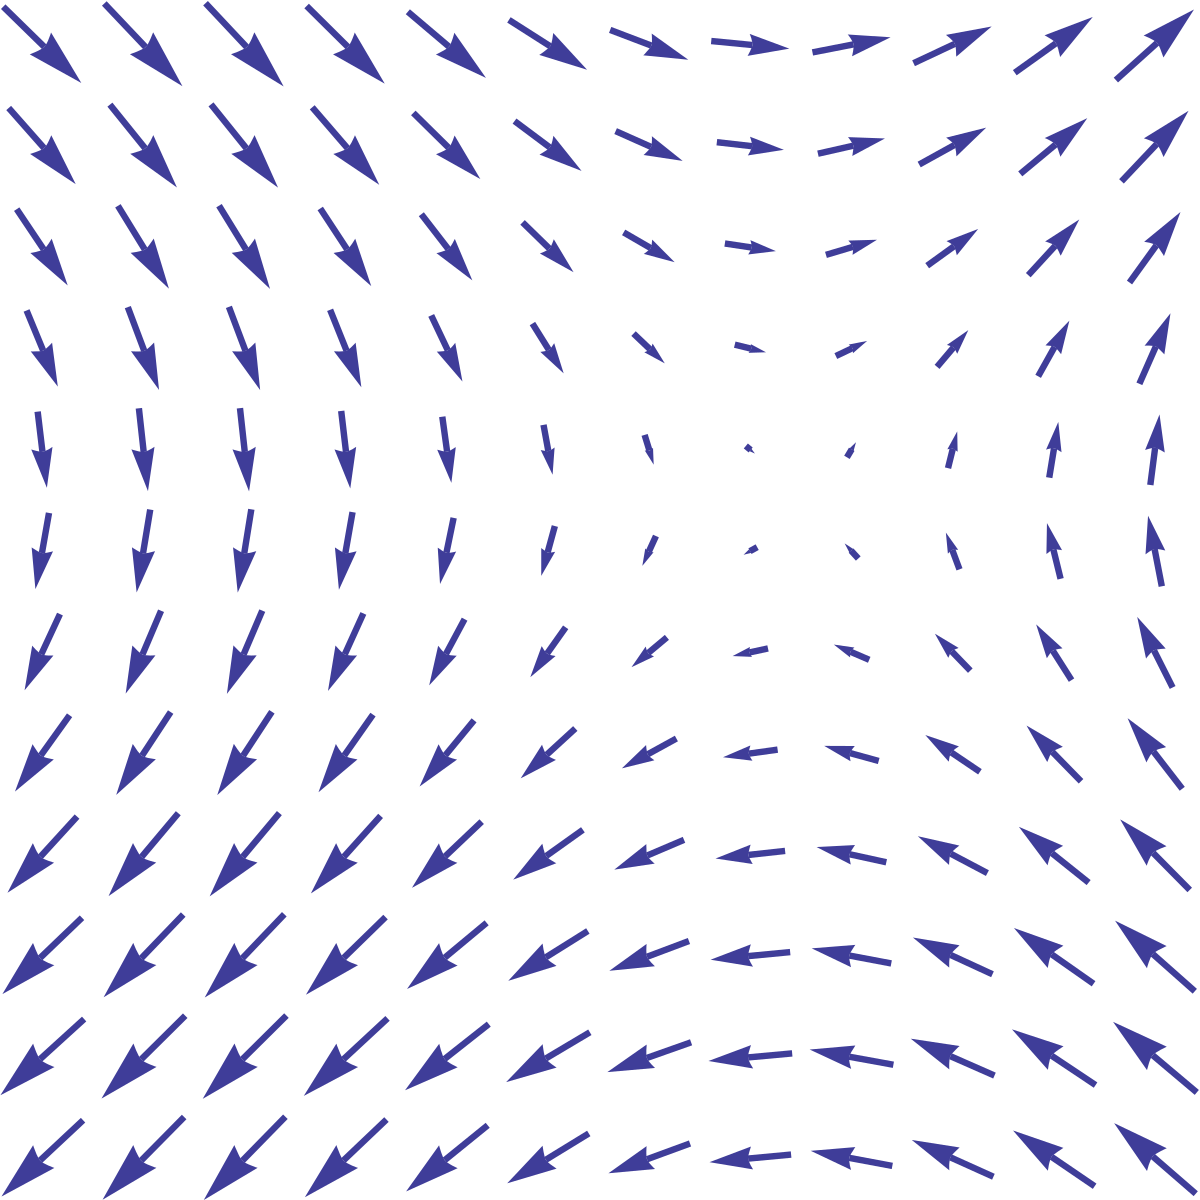
\includegraphics[width=\textwidth]{figures/vectorField.png}
\caption{\label{fig:field} A vector field of vectors $\vec{v}_{\rm i}$.  Let $\hat{j}$ represent up, and $\hat{i}$ represent right.}
\end{figure}
\end{column}
\end{columns}
\end{frame}

\begin{frame}{Coulomb’s Law and Electric Fields}
\small
\begin{columns}[T]
\begin{column}{0.5\textwidth}
Which of the following is true of vectors $\vec{v}_{\rm i}$ in the upper left-hand corner of the figure at right?
\begin{itemize}
\item A: They are probably $\vec{v}_{\rm i} = -\hat{i}-\hat{j}$
\item B: They are probably $\vec{v}_{\rm i} = \hat{i}+\hat{j}$
\item C: They are probably $\vec{v}_{\rm i} = -\hat{i}+\hat{j}$
\item D: They are probably $\vec{v}_{\rm i} = \hat{i}-\hat{j}$
\end{itemize}
\end{column}
\begin{column}{0.5\textwidth}
\begin{figure}
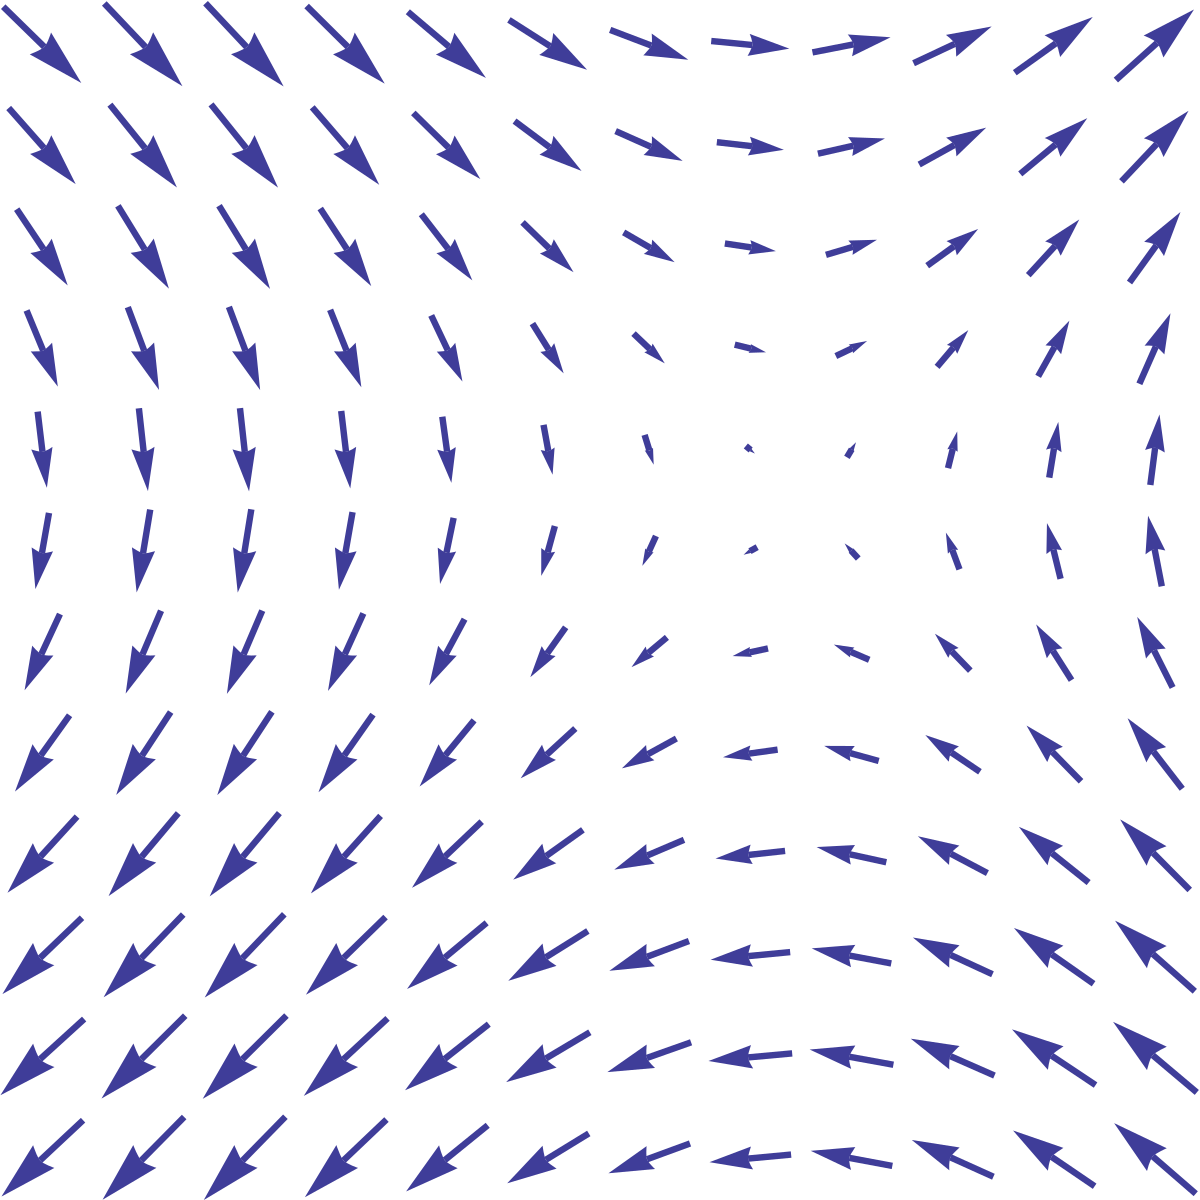
\includegraphics[width=\textwidth]{figures/vectorField.png}
\caption{\label{fig:field2} A vector field of vectors $\vec{v}_{\rm i}$.  Let $\hat{j}$ represent up, and $\hat{i}$ represent right.}
\end{figure}
\end{column}
\end{columns}
\end{frame}

\begin{frame}{Coulomb’s Law and Electric Fields}
\small
\begin{columns}[T]
\begin{column}{0.5\textwidth}
\textbf{Group board exercise}: What is the angle of the net electric field for the \textit{test charge} at the point (1,1) in Fig. \ref{fig:netfield1}? \\ \vspace{0.5cm}
\textbf{Group board exercise}: What is the magnitude of the net electric field for the \textit{test charge} at the point (1,1) in Fig. \ref{fig:netfield1}, if the distances have units of nanometers, and $q$ is the charge of an electron, $1.6\times 10^{-19}$ C? (Let $\frac{1}{4\pi\epsilon_{\rm 0}} = 9\times 10^{9}$ N m$^2$ C$^{-2}$).\\ \vspace{0.5cm}
\end{column}
\begin{column}{0.5\textwidth}
\begin{figure}
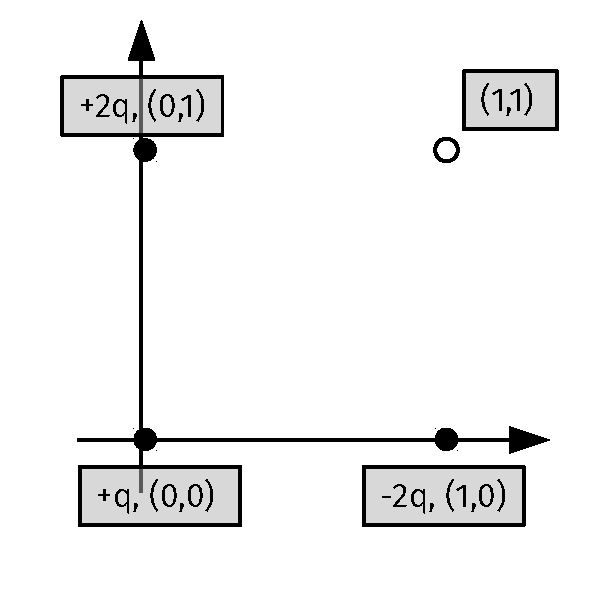
\includegraphics[width=\textwidth]{figures/NetField1.pdf}
\caption{\label{fig:netfield1} Three charges create a field for a hypothetical \textit{test charge}.}
\end{figure}
\end{column}
\end{columns}
\end{frame}

\begin{frame}{Coulomb’s Law and Electric Fields}
\small
\begin{columns}[T]
\begin{column}{0.5\textwidth}
What is the angle of the E-field at point (1,1) in Fig. \ref{fig:netfield2} at right?
\begin{itemize}
\item A: 0 deg
\item B: 45 deg
\item C: 90 deg
\item D: 135 deg
\end{itemize}
What is the fastest way to solve this problem?
\begin{itemize}
\item A: Blind luck
\item B: Do the algebra
\item C: Symmetry
\item D: Numerical estimation
\end{itemize}
\end{column}
\begin{column}{0.5\textwidth}
\begin{figure}
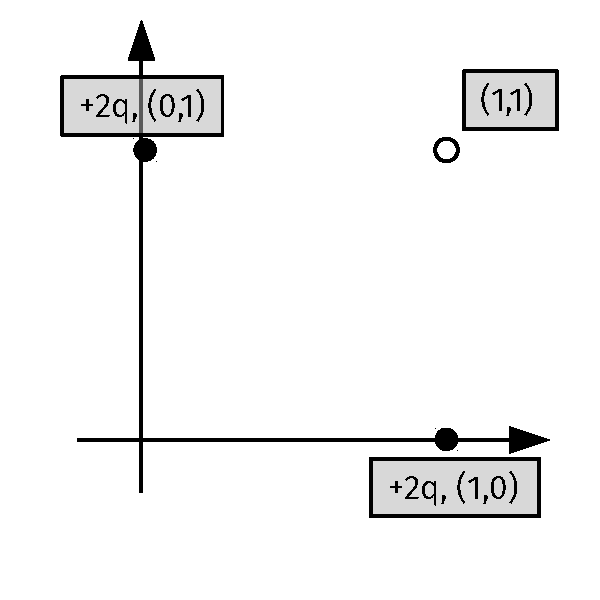
\includegraphics[width=\textwidth]{figures/NetField2.pdf}
\caption{\label{fig:netfield2} Two charges create a field for a hypothetical \textit{test charge}.}
\end{figure}
\end{column}
\end{columns}
\end{frame}

\begin{frame}{Coulomb’s Law and Electric Fields}
\small
\begin{columns}[T]
\begin{column}{0.5\textwidth}
What is the angle of the E-field at point (1,1) in Fig. \ref{fig:netfield3} at right?
\begin{itemize}
\item A: About 0 deg
\item B: About 25 deg
\item C: About 45 deg
\item D: About 60 deg
\end{itemize}
\end{column}
\begin{column}{0.5\textwidth}
\begin{figure}
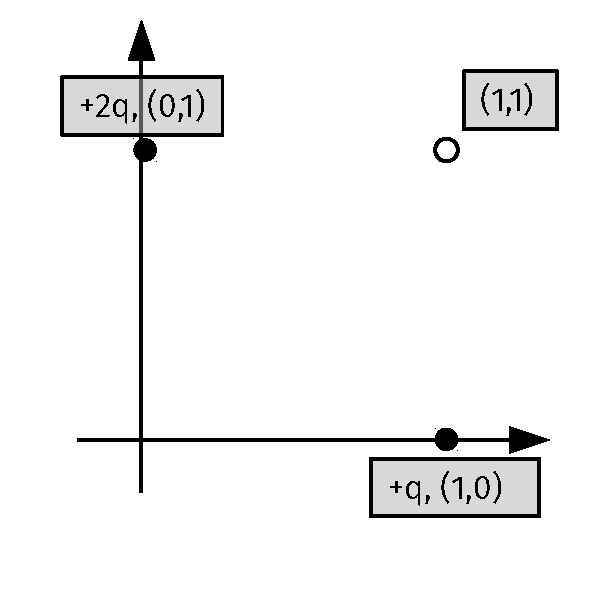
\includegraphics[width=\textwidth]{figures/NetField3.pdf}
\caption{\label{fig:netfield3} Two charges create a field for a hypothetical \textit{test charge}.}
\end{figure}
\end{column}
\end{columns}
\end{frame}

\begin{frame}{Coulomb’s Law and Electric Fields}
The forces of $N$ fixed charges on a test charge $Q$ create a net force, where the individual forces simply add like vectors.  This is known as the \textbf{superposition principle}.
\begin{align}
\vec{F}_{\rm C,Net} &= \frac{1}{4\pi\epsilon_{\rm 0}} Q \sum_{i = 1}^N \frac{q_i}{r_i^2}\hat{r}_i = Q \vec{E}_{\rm C,Net} \\
\vec{E}_{\rm C,Net} &= \frac{1}{4\pi\epsilon_{\rm 0}} \sum_{i = 1}^N \frac{q_i}{r_i^2}\hat{r}_i
\end{align}
\end{frame}

\begin{frame}{Coulomb’s Law and Electric Fields}
For the expressions of fields built from the superposition principle, let's adopt a notation:
\begin{equation}
\vec{E}_{\rm C,Net}(P) = \frac{1}{4\pi\epsilon_{\rm 0}} \sum_{i = 1}^N \frac{q_i}{r_i^2}\hat{r}_i \label{eq:P}
\end{equation}
Equation \ref{eq:P} represents the field at a \textit{position} $P = P(x,y,z)$, relative to the positions $\vec{r}_i$ of the source charges.
\end{frame}

\begin{frame}{Coulomb’s Law and Electric Fields}
\small
\begin{columns}[T]
\begin{column}{0.5\textwidth}
\textbf{Table exercise:} Calculate $\vec{E}_{\rm C,Net}(P)$, if $P = (1,1)$. \\ \vspace{0.5cm}
\textbf{Table exercise:} Calculate $\vec{E}_{\rm C,Net}(P)$, if $P = (-1,-1)$. \\ \vspace{0.5cm}
\textbf{Group discussion:} What does it mean if $P = (1,0)$? \\ \vspace{0.5cm}
\end{column}
\begin{column}{0.5\textwidth}
\begin{figure}
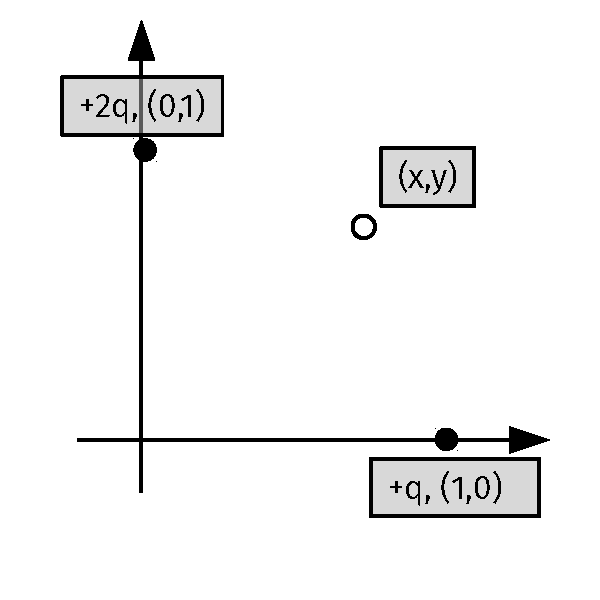
\includegraphics[width=\textwidth]{figures/NetField4.pdf}
\caption{\label{fig:netfield4} Two charges create a field for a hypothetical \textit{test charge}.}
\end{figure}
\end{column}
\end{columns}
\end{frame}

\begin{frame}{Coulomb’s Law and Electric Fields}
Notice in the prior examples of \textit{fixed} charges, we need an \textit{explanation} for why the fixed charges remain fixed, even though they are obviously subject to Coulomb forces. \\ \vspace{0.5cm}
\textbf{Insulator}: A material in which there are no free charges available to conduct electricity.  Charges may be fixed in position within an insulator. \\
\textbf{Conductor}: A material in which there are free charges available to conduct electricity.  Charges may not be fixed in position within a conductor. \\
\textbf{Semi-conductor}: A material in which there are free charges available to conduct electricity if certain requirements are met.
\end{frame}

\begin{frame}{Coulomb’s Law and Electric Fields}
\small
\begin{columns}[T]
\begin{column}{0.5\textwidth}
The following problem is an example of solving for a field analytically, and \textit{testing various limits}.  Upon taking limits results are often simple and intuitive. \\ \vspace{0.5cm}
Two charges $+q$ are on the fixed in an insulator on the x-axis.  Solve for the E-field at $P = (0,0,z)$. \\ \vspace{0.5cm}
Show that the general solution is
\begin{equation}
\vec{E}(z) = \frac{1}{4\pi\epsilon_0} \frac{2qz}{\left(z^2+\left(\frac{d}{2}\right)^2\right)^{3/2}} \hat{k}
\end{equation}
\end{column}
\begin{column}{0.5\textwidth}
\begin{figure}
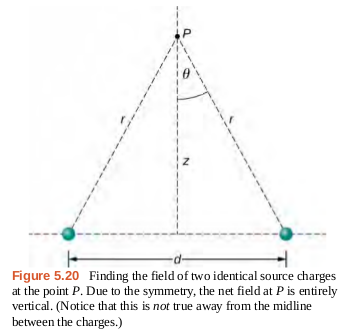
\includegraphics[width=\textwidth]{figures/twoChargesZ.png}
\caption{\label{fig:twoChargesZ} Solve for the E-field as a function of $z$, $d$, and $q$.}
\end{figure}
\end{column}
\end{columns}
\end{frame}

\begin{frame}{Coulomb’s Law and Electric Fields}
\small
\begin{columns}[T]
\begin{column}{0.5\textwidth}
Show that the general solution is
\begin{equation}
\vec{E}(z) = \frac{1}{4\pi\epsilon_0} \frac{2qz}{\left(z^2+\left(\frac{d}{2}\right)^2\right)^{3/2}} \hat{k}
\end{equation}
\textit{Take the following two limits:} \\ 1) $z \gg d$ and 2) $z=0$.  What are the results? \\ \vspace{0.5cm}
Keep these results in mind, because we are about to start drawing \textbf{vector fields,} in order to visualize the algebra.
\end{column}
\begin{column}{0.5\textwidth}
\begin{figure}
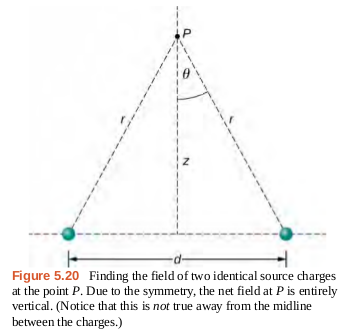
\includegraphics[width=\textwidth]{figures/twoChargesZ.png}
\caption{\label{fig:twoChargesZ2} Solve for the E-field as a function of $z$, $d$, and $q$.}
\end{figure}
\end{column}
\end{columns}
\end{frame}

\begin{frame}{Coulomb’s Law and Electric Fields}
\textbf{PhET Simulation of E-fields from Charges}: \\ \vspace{0.5cm}
\url{https://phet.colorado.edu/en/simulation/charges-and-fields}
\begin{enumerate}
\item Create the situation in the prior problem, in Fig. \ref{fig:twoChargesZ2}.
\item Use the yellow sensor object to determine the local direction of the E-field at various points along the z-axis.
\begin{itemize}
\item Do the results match the limit $z\gg d$?
\item Do the results match the limit $z = 0$, halfway between the charges?
\item Where is the field maximal?
\end{itemize}
\item Make sure you can see above and below the charges, and repeat steps 1 and 2 for negative z-values.  What do you find?
\end{enumerate}
\end{frame}

\begin{frame}{Coulomb’s Law and Electric Fields}
\small
\textbf{PhET Simulation of E-fields from Charges}: \\ \vspace{0.5cm}
Build E-fields with the following properties, by adding single charges.  Let the \textit{z-axis be upwards}, and let the \textit{x-axis be to the right.}
\begin{enumerate}
\item Build an electric field that has \textbf{reflection symmetry} across the z-axis, with at least five charges.
\item Build an electric field that has \textit{radial symmetry} about the origin, with at least six charges.
\item Build an electric field that would be the same if I rotated the picture by 90 degrees (\textbf{4-fold symmetry}) with at least four charges, some negative and some positive.
\item Build an electric field that would be the same if I rotated the picture by 45 degrees (\textbf{8-fold symmetry}) with at least eight charges, some negative and some positive.
\end{enumerate}
\end{frame}

\begin{frame}{Coulomb’s Law and Electric Fields}
\small
\textbf{PhET Simulation of E-fields from Charges}: \\ \vspace{0.5cm}
\alert{The lesson is that the E-field has the \textit{symmetry properties} of the \textit{charge distribution}}.
\end{frame}

\begin{frame}{Coulomb’s Law and Electric Fields}
When we connect the vectors in a vector field, the results are figures like Fig. \ref{fig:lines}.  Fields by convention originate from positive charges and terminate on negative ones.
\begin{figure}
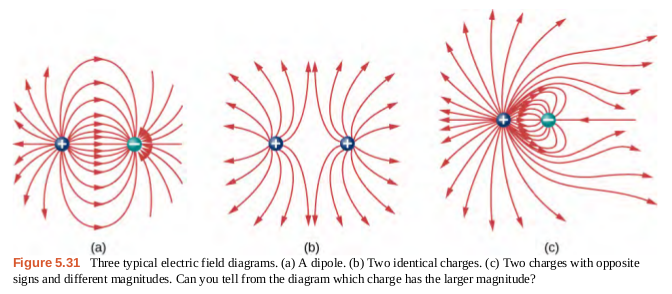
\includegraphics[width=0.8\textwidth]{figures/lines.png}
\caption{\label{fig:lines} Field-line diagrams.  The density of lines indicates electric field strength.}
\end{figure}
\end{frame}

\section{E-Fields of Charge Distributions}

\begin{frame}{E-Fields of Charge Distributions}
Welcome to calculus! Let $k = 1/(4\pi\epsilon_0)$.
\begin{align}
\vec{E}(P) &= k \sum_{i = 1}^N \left(\frac{q_i}{r_i^2}\right) \hat{r} \label{eq:point} \\
\vec{E}(P) &= k \int_{line} \left(\frac{\lambda dl}{r^2}\right) \hat{r} \label{eq:line} \\
\vec{E}(P) &= k \int_{surface} \left(\frac{\sigma dA}{r^2}\right) \hat{r} \label{eq:surface} \\
\vec{E}(P) &= k \int_{volume} \left(\frac{\rho dV}{r^2}\right) \hat{r} \label{eq:volume}
\end{align}
The functions $\lambda$, $\sigma$, and $\rho$ are just charge densities.  They decribe where charge is, and how much there is.  
\end{frame}

\begin{frame}{E-Fields of Charge Distributions}
\begin{figure}
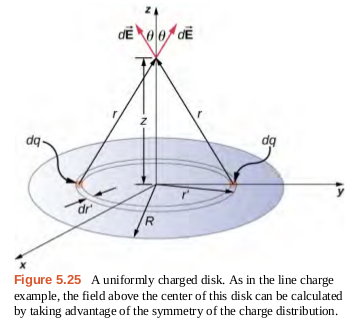
\includegraphics[width=0.45\textwidth]{figures/disk.png}
\caption{\label{fig:disk} We are going to work this example together, and other examples will be left to homework.}
\end{figure}
\textbf{Observe on board.}
\end{frame}

\begin{frame}{E-Fields of Charge Distributions}
\begin{figure}
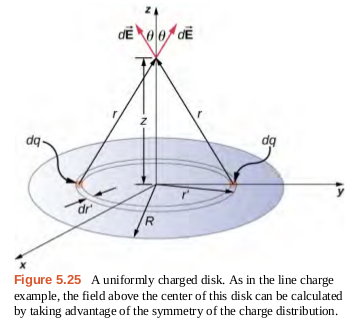
\includegraphics[width=0.4\textwidth]{figures/disk.png}
\caption{\label{fig:disk2} We are going to work this example together, and other examples will be left to homework.}
\end{figure}
Result:
\begin{equation}
\boxed{
\vec{E} = k\left(2\pi\sigma - \frac{2\pi\sigma z}{\sqrt{R^2 + z^2}} \right)\hat{k}}
\end{equation}
\end{frame}

\begin{frame}{E-Fields of Charge Distributions}
\begin{equation}
\boxed{
\vec{E} = k\left(2\pi\sigma - \frac{2\pi\sigma z}{\sqrt{R^2 + z^2}} \right)\hat{k}} \label{eq:disk}
\end{equation}
Which of the following not true of Eq. \ref{eq:disk}?
\begin{itemize}
\item A: Taking the limit $R \rightarrow \infty$ yields a constant field.
\item B: Taking the limit $z \rightarrow 0$ yields a constant field.
\item C: The charge distribution has radial symmetry, so the field cannot have horizontal components.
\item D: Taking the value $z = R$ represents a minimum in the field strength.
\end{itemize}
\end{frame}

\begin{frame}{E-Fields of Charge Distributions}
\begin{equation}
\boxed{
\vec{E} = k\left(2\pi\sigma - \frac{2\pi\sigma z}{\sqrt{R^2 + z^2}} \right)\hat{k}} \label{eq:disk2}
\end{equation}
What happens to Eq. \ref{eq:disk2}, in the limit that $R \rightarrow \infty$?
\begin{itemize}
\item A: The field decreases to zero.
\item B: The field is constant.
\item C: The field grows increasingly positive.
\item D: The field grows increasingly negative.
\end{itemize}
\end{frame}

\begin{frame}{E-Fields of Charge Distributions}
In the limit that $R \rightarrow \infty$,
\begin{equation}
\vec{E} = 2\pi\sigma k \hat{k} = \frac{\sigma}{2\epsilon_0} \hat{k} \label{eq:disk3}
\end{equation}
Equation for the electric field of a uniform infinite disk.
\end{frame}

\begin{frame}{E-Fields of Charge Distributions}
Imagine two infinite disks with equal uniform charge distributions, some distance apart.  One has positive charge, the other negative charge.  What is the E-field between them?
\begin{itemize}
\item A: 0
\item B: $\frac{\sigma}{2\epsilon_0}$
\item C: $\frac{\sigma}{\epsilon_0}$
\item D: $\frac{\sigma}{4\epsilon_0}$
\end{itemize}
\end{frame}

\begin{frame}{E-Fields of Charge Distributions}
Imagine two infinite disks with equal uniform charge distributions, some distance apart.  Both have positive charge.  What is the E-field between them?
\begin{itemize}
\item A: 0
\item B: $\frac{\sigma}{2\epsilon_0}$
\item C: $\frac{\sigma}{\epsilon_0}$
\item D: $\frac{\sigma}{4\epsilon_0}$
\end{itemize}
\end{frame}

\begin{frame}{E-Fields of Charge Distributions}
Other interesting charge distributions:
\begin{itemize}
\item A line of charge with length $L$ and total charge $Q = \lambda L$, where $P = (0,0,z)$ above midpoint:
\begin{equation}
\vec{E}(z) = \frac{1}{4\pi\epsilon_0} \frac{\lambda L}{z\sqrt{z^2 + \frac{1}{4} L^2}} \hat{k} \label{eq:line2}
\end{equation}
\item Equation \ref{eq:line2}, but with $L \rightarrow \infty$:
\begin{equation}
\vec{E}(z) = \frac{1}{4\pi\epsilon_0} \frac{2\lambda}{z} \hat{k}
\end{equation}
\end{itemize}
\end{frame}

\begin{frame}{E-Fields of Charge Distributions}
Other interesting charge distributions:
\begin{itemize}
\item A ring of radius $R$ and total charge $Q = 2\pi R\lambda$, where $P = (0,0,z)$ above midpoint:
\begin{equation}
\vec{E}(z) = \frac{1}{4\pi\epsilon_0} \frac{2\pi R \lambda z}{\left(z^2 + R^2\right)^{3/2}} \hat{k} \label{eq:ring}
\end{equation}
\item Equation \ref{eq:ring}, but with $z \gg R$:
\begin{equation}
\vec{E}(z) = \frac{1}{4\pi\epsilon_0} \frac{2\pi R \lambda }{z^2} \hat{k} \label{eq:ring2}
\end{equation}
\end{itemize}
\end{frame}

\begin{frame}{E-Fields of Charge Distributions}
In Eq. \ref{eq:ring}, what does the quantity $2\pi R\lambda$ represent?
\begin{itemize}
\item A: The total charge density on the ring
\item B: The circumference of the ring
\item C: The magnitude of the electric field from the ring
\item D: The total charge on the ring
\end{itemize}
\end{frame}

\begin{frame}{E-Fields of Charge Distributions}
Let $Q_{\rm tot} = 2\pi R \lambda$.  That makes Eq. \ref{eq:ring2}
\begin{equation}
\vec{E}(z) = \frac{1}{4\pi\epsilon_0} \frac{Q_{\rm tot}}{z^2} \hat{k}
\end{equation}
This is identical to the electric field of what charge distribution?  (Think back to the definition of the electric field).
\begin{itemize}
\item A: A plane with charge density $Q_{\rm tot}/A$, where $A$ is the area
\item B: A line with total charge $Q_{\rm tot}$
\item C: A dipole of charge $\pm Q_{\rm tot}$
\item D: A point charge $Q_{\rm tot}$
\end{itemize}
\end{frame}

\section{Electric Potential, Potential Energy}

\begin{frame}{Electric Potential, Potential Energy}
Recall that the \textit{change in potential energy} is force:
\begin{equation}
F = -\frac{\Delta U}{\Delta x}
\end{equation}
\begin{itemize}
\item The units of $U$: Joules = Newtons per meter
\item The units of $x$: meters
\item The ratio: Newtons
\end{itemize}
\end{frame}

\begin{frame}{Electric Potential, Potential Energy}
An object of mass $m$ is a height $h$ above the ground, in Earth's gravity field.  What is the \textit{potential} energy of the object?
\begin{itemize}
\item A: $U = \frac{1}{2}mv^2$ ($v$ is the velocity)
\item B: $U = \frac{1}{2}mv^2 + mgh$ ($v$ is the velocity)
\item C: $U = mgh$
\item D: $U$ is zero, because the object is at rest.
\end{itemize}
\end{frame}

\begin{frame}{Electric Potential, Potential Energy}
What is the expression for the force of gravity, if $\Delta U = mgh$, and $\Delta x = h$?
\begin{itemize}
\item A: $mg$
\item B: $-mg$
\item C: $g$
\item D: $-g$
\end{itemize}
\end{frame}

\begin{frame}{Electric Potential, Potential Energy}
\small
If the potential energy is a function of displacement, $U = U(\vec{x})$, it may be called a potential energy \textit{surface}.
\begin{figure}
\centering
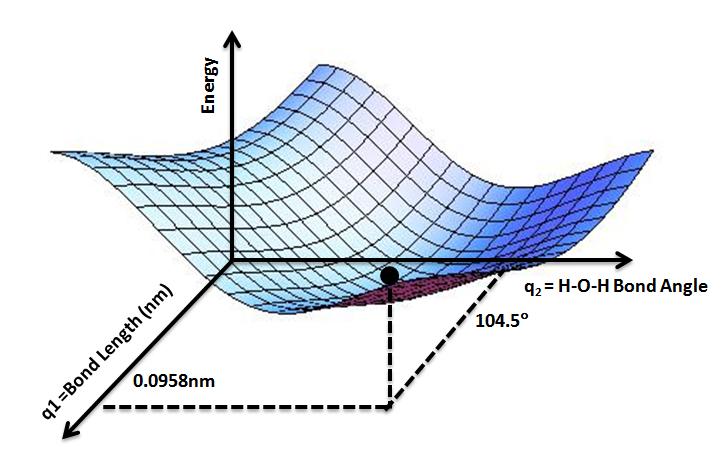
\includegraphics[width=0.5\textwidth]{figures/potential.png}
\caption{\label{fig:potential} An example of a potential energy surface.}
\end{figure}
\end{frame}

\begin{frame}{Electric Potential, Potential Energy}
\small
Considering \textit{Newton's Second Law}, however, if $F = m a$ then $m a = -\frac{\Delta U}{\Delta x}$, and
\begin{equation}
a = -\frac{1}{m}\frac{\Delta U}{\Delta x}
\end{equation}
\begin{figure}
\centering
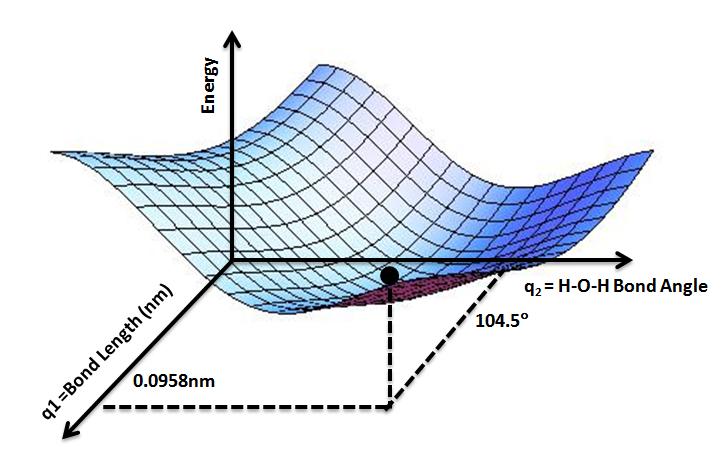
\includegraphics[width=0.5\textwidth]{figures/potential.png}
\caption{\label{fig:potential2} \small Imagine dividing the numbers on the z-axis by the mass, and treating this surface as the potential energy \textit{per unit mass}.}
\end{figure}
\end{frame}

\begin{frame}{Electric Potential, Potential Energy}
\small
Let's just scale the z-axis by the mass of the system:
\begin{align}
a &= -\frac{1}{m}\frac{\Delta U}{\Delta x} \\
\Delta V &= \frac{\Delta U}{m} \\
a &= -\frac{\Delta V}{\Delta x}
\end{align}
Instead of calling $\Delta V$ the potential energy, let's just call it \textit{the potential.}  Recall that if the force is a vector field, then acceleration is a vector field as well (the object has a given acceleration vector for all points in the space).
\end{frame}

\begin{frame}{Electric Potential, Potential Energy}
\begin{columns}[T]
\begin{column}{0.5\textwidth}
\alert{Newtonian mechanics} \\ \hrulefill
\begin{align}
F &= ma \\
a &= -\frac{\Delta V}{\Delta x}
\end{align}
\end{column}
\begin{column}{0.5\textwidth}
\alert{Electrostatics} \\ \hrulefill
\begin{align}
F &= qE \\
E &= -\frac{\Delta V}{\Delta x} \label{eq:volt}
\end{align}
\end{column}
\end{columns} \vspace{1cm}
In Eq. \ref{eq:volt}, we refer to $\Delta V$ as \textbf{voltage.}
\end{frame}

\begin{frame}{Electric Potential, Potential Energy}
\textbf{Good paper topic:}
\begin{figure}
\centering

\includegraphics[width=0.4\textwidth]{figures/volta.jpg}
\caption{\label{fig:volta} \small (Lago di Como, Italia) Monument to Alessandro Volta, inventor of the electric battery.  Debunked claim that electricity only generated by life.}
\end{figure}
\end{frame}

\begin{frame}{Electric Potential, Potential Energy}
\textbf{Voltage} is like a potential energy surface $\rightarrow$ \textit{potential energy per unit charge.} \\ \vspace{0.5cm}
\url{https://phet.colorado.edu/en/simulation/charges-and-fields} \\
\alert{Using the PhET simulation about charges and fields}:
\begin{enumerate}
\item Explore the voltage associated with fields generated by charges using the voltage button.
\item Add a single point charge, and use the ruler and voltmeter (potentiometer) to measure voltage versus distance, and plot it.
\item What function describes the relationship between voltage and distance?
\end{enumerate}
\end{frame}

\begin{frame}{Electric Potential, Potential Energy}
\url{https://phet.colorado.edu/en/simulation/charges-and-fields} \\
\alert{Using the PhET simulation about charges and fields}:
\begin{enumerate}
\item Note that the units of $\epsilon_0$ are N m$^2$ C$^{-2}$, and the value is $8.854\times 10^{-12}$
\item We know from prior equations that the units of voltage are J C$^{-1}$
\item Using your measurements, show that the voltage due to a point charge is
\begin{equation}
\boxed{
V = \pm \frac{1}{4\pi \epsilon_0} \frac{q}{r}}
\end{equation}
(Where the sign depends on the charge, just like E-fields)
\end{enumerate}
\end{frame}

\begin{frame}{Electric Potential, Potential Energy}
Voltage due to a point charge:
\begin{equation}
\boxed{
V = \pm \frac{1}{4\pi \epsilon_0} \frac{q}{r}} \label{eq:volt2}
\end{equation}
Equation \ref{eq:volt2} follows from the form of the electric field of a point charge, and $E = -\Delta V/\Delta x$ (derivative, calculus).
\end{frame}

\begin{frame}{Electric Potential, Potential Energy}
Voltage is an example of a \textbf{scalar field}, whereas the electric field is an example of a \textbf{vector field.}  Recall the result for the electric field of a large plane of charge, with charge $\sigma$ per unit area:
\begin{equation}
\vec{E} = \frac{\sigma}{2\epsilon_0} \hat{k}
\end{equation}
What should the voltage be, if the field is constant?  (Think of the situation of gravity, with electric field standing in for acceleration). \\ \vspace{0.5cm}
\url{https://phet.colorado.edu/en/simulation/charges-and-fields}
\end{frame}

\begin{frame}{Electric Potential, Potential Energy}
\begin{figure}
\centering
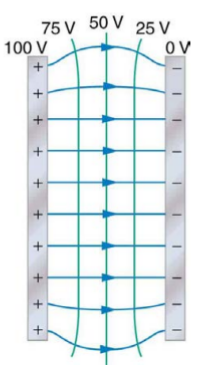
\includegraphics[width=0.25\textwidth]{figures/plates.png}
\caption{\label{fig:plates} Parallel plates of charge, electric field, and potential.  Notice the linear decrease in voltage.  Did you see this in the PhET?}
\end{figure}
\end{frame}

\begin{frame}{Electric Potential, Potential Energy}
\textit{Two parallel plates, opposite charge}:
\begin{equation}
V = -\frac{\sigma}{\epsilon_0}z + C
\end{equation}
With the boundary condition that $V = V_0$ when $z = 0$, we have
\begin{equation}
V(z) - V_0 = -\frac{\sigma}{\epsilon_0}z
\end{equation}
Let $\Delta V(z) = V(z) - V_0$, and $\Delta z = z$:
\begin{equation}
\frac{\Delta V}{\Delta z} = -\frac{\sigma}{\epsilon_0} =  E
\end{equation}
\end{frame}

\section{Voltage, Potential Energy, and Work}

\begin{frame}{Voltage, Potential Energy, and Work}
\small
What follows is a series of memorizable equations and mental images comparing voltage to gravitational potential energy.  This analogy runs deep because the Coulomb force is conservative.
\begin{figure}
\centering
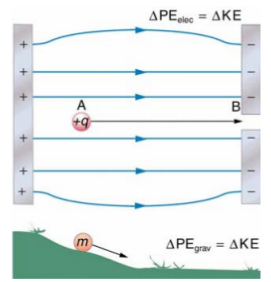
\includegraphics[width=0.45\textwidth]{figures/hill.png}
\caption{\label{fig:hill} Remembering the connection of voltage to gravity.}
\end{figure}
\end{frame}

\begin{frame}{Voltage, Potential Energy, and Work}
We can think of work as the opposite in the change in potential energy: $W = -\Delta PE$.  If gravity pulls an object down a hill, that object is losing gravitational potential energy, and the energy is being converted to kinetic energy.  Which of the following formulas describes the relationship between work and displacement?
\begin{itemize}
\item A: $W = \vec{F} \cdot \vec{x} = Fx\cos\theta$
\item B: $W = \frac{\Delta F}{\Delta x}$
\item C: $W = mgx F$
\item D: I'm confused.
\end{itemize}
\end{frame}

\begin{frame}{Voltage, Potential Energy, and Work}
Imagine trying to calculate the work done ($W = -\Delta PE$) on a charge $q$ as it moves through a complex vector field ($F = qE$, where $E$ can come from some complex charge distribution).  It's easier to take the test charge $q$ out of it, and think of just the potential surface as a surface, rather than proportional to $qE$ times the path.
\begin{equation}
V = \frac{PE}{q}
\end{equation}
This makes the unit of one Volt equal to one Joule per Coulomb. (1 V = 1 J/C).  The volt reminds us of all those times the \textit{mass drops out} of the problems when we are not concerned with how many Newtons, just where things are going.
\end{frame}

\begin{frame}{Voltage, Potential Energy, and Work}
For potential energy calculations involving gravity, \textbf{we} get to decide the location of ``zero energy,'' and we're only interested in \textit{changes} in potential energy.
\begin{equation}
\Delta V = V_{\rm B} - V_{\rm A} = \frac{\Delta PE}{q}
\end{equation}
Where is the most logical place to put the voltage zero point?
\end{frame}

\begin{frame}{Voltage, Potential Energy, and Work}
\begin{figure}
\centering
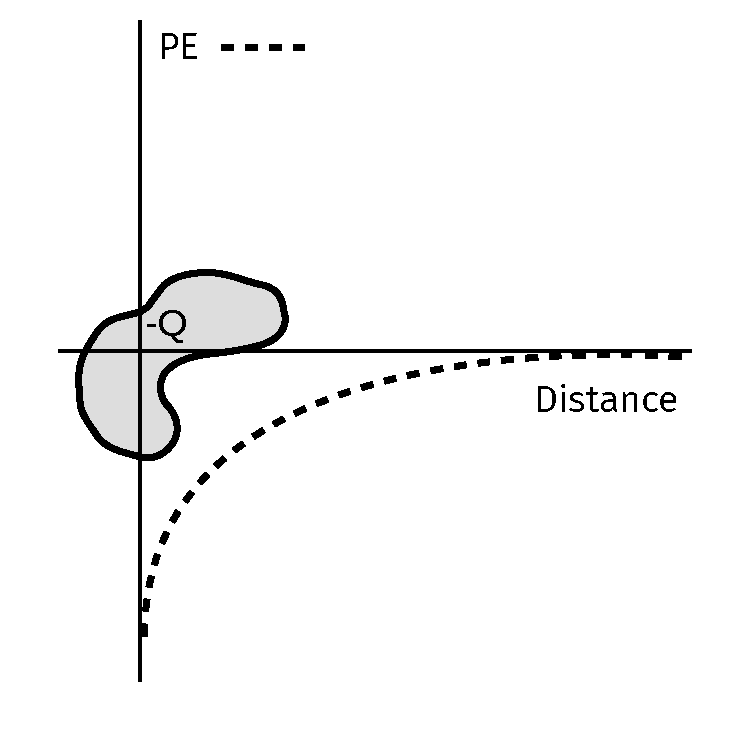
\includegraphics[width=0.6\textwidth]{figures/PE.pdf}
\caption{\label{fig:PE} Where should we place the zero point of potential energy here?  Which way do positive charges fall?  Which way do negative charges fall?}
\end{figure}
\end{frame}

\begin{frame}{Voltage, Potential Energy, and Work}
\begin{figure}
\centering
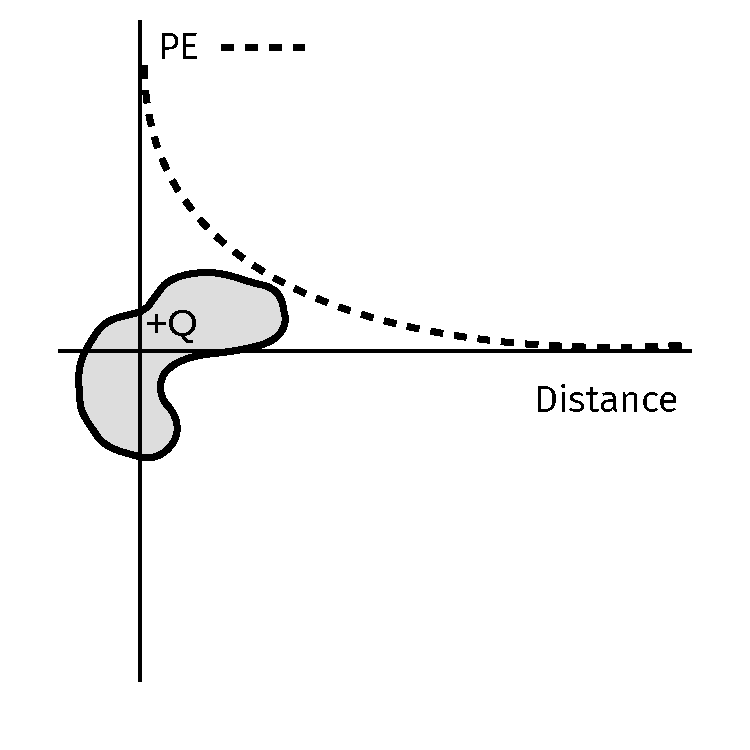
\includegraphics[width=0.6\textwidth]{figures/PE2.pdf}
\caption{\label{fig:PE2} Where should we place the zero point of potential energy here?  Which way do positive charges fall?  Which way do negative charges fall?}
\end{figure}
\end{frame}

\begin{frame}{Voltage, Potential Energy, and Work}
Suppose you have a 12.0 V motorcycle battery that can move 5000 C of charge, and a 12.0 V car battery that can move 60,000 C of charge. How much energy does each deliver?
\begin{itemize}
\item A: 60 kJ and 720 kJ, respectively
\item B: 600 kJ and 7200 kJ, respectively
\item C: 6 kJ and 72 kJ, respectively
\item D: 0.6 kJ and 7.2 kJ, respectively
\end{itemize}
\end{frame}

\begin{frame}{Voltage, Potential Energy, and Work}
\begin{figure}
\centering
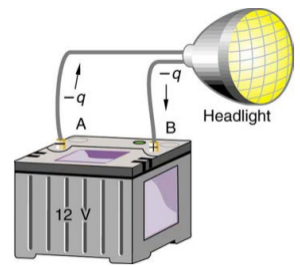
\includegraphics[width=0.6\textwidth]{figures/headlight.png}
\caption{\label{fig:headlight.png} Here is a battery circuit that has a potential difference of 12 V.  Where would you put the zero point?}
\end{figure}
\end{frame}

\begin{frame}{Voltage, Potential Energy, and Work}
Consider the battery headlight circuit.  The car batter has 60,000 C stored, with $\Delta V = 12.0$ V.  The headlight requires 30 W of power.  We know how much energy is in the battery, so how long can the headlight run?
\begin{itemize}
\item A: About 1 hour
\item B: About 2 hours
\item C: About 7 hours
\item D: About 9 hours
\end{itemize}
\end{frame}

\begin{frame}{Voltage, Potential Energy, and Work}
\textbf{Smaller than a motorcycle battery}: Suppose an AA battery has 1.5 V, and 7200 C of charge.  How much energy is stored inside it?
\begin{itemize}
\item A: About 5 kJ
\item B: About 10 kJ
\item C: About 15 kJ
\item D: About 20 kJ
\end{itemize}
\end{frame}

\begin{frame}{Voltage, Potential Energy, and Work}
Same headlight: requires 30 W of power.  We know how much energy is in the battery, so how long can the headlight run?
\begin{itemize}
\item A: About 1 hour
\item B: About 30 minutes
\item C: About 15 minutes
\item D: About 6 minutes
\end{itemize}
\end{frame}

\begin{frame}{Voltage, Potential Energy, and Work}
\textbf{Scaling problems:} Consider two batteries.  Battery 1 has 5000 C at 12 V.  Battery 2 has the same charge but only 3/4 the energy.  What is the voltage of battery 2?
\begin{itemize}
\item A: 5 V 
\item B: 7 V
\item C: 9 V
\item D: 12 V
\end{itemize}
\end{frame}

\begin{frame}{Voltage, Potential Energy, and Work}
\textbf{Scaling problems:} Two AA batteries have 1.5 V each.  Placed end-to-end, the voltages add together.  If each had 7200 C of charge, what's the new energy of the double battery system?
\begin{itemize}
\item A: 5 kJ
\item B: 10 kJ
\item C: 15 kJ
\item D: 20 kJ
\end{itemize}
\end{frame}

\begin{frame}{Voltage, Potential Energy, and Work}
\textbf{Scaling problems:} A 24V solar-cell battery can run a 10 W system for 24 hours.  If we add a second 24V battery with half the charge of the first, for how long can the system run?
\begin{itemize}
\item A: 24 hours
\item B: 36 hours
\item C: 48 hours
\item D: 12 hours
\end{itemize}
\end{frame}

\begin{frame}{Voltage, Potential Energy, and Work}
\textbf{The electron-Volt, eV}: Since charge times voltage is energy, why not have a unit where it's the charge of one electron through a potential difference of one volt? \\ \vspace{0.5cm}
$q_{\rm e} \approx 1.6 \times 10^{-19}$ C, 1 eV = $1.6 \times 10^{-19}$ J. \\ \vspace{0.5cm}
This unit comes in handy!
\end{frame}

\begin{frame}{Voltage, Potential Energy, and Work}
\begin{figure}
\centering
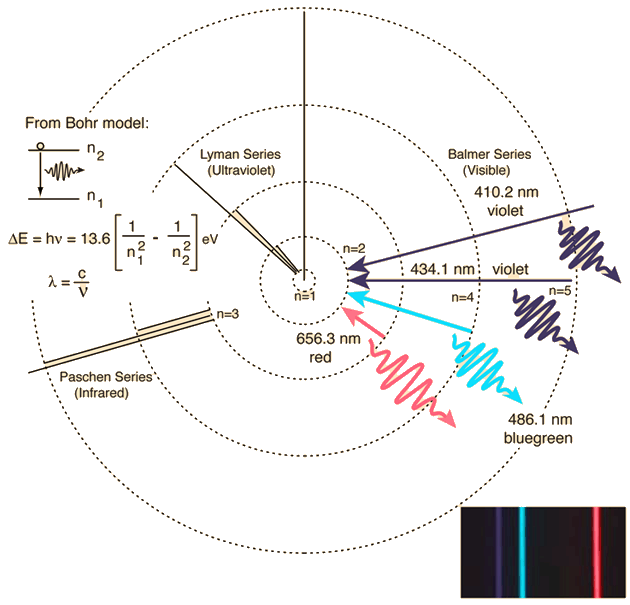
\includegraphics[width=0.65\textwidth]{figures/H.png}
\caption{\label{fig:H} Energies of order 1 electron-Volt. Our whole visual range...}
\end{figure}
\end{frame}

\begin{frame}{Voltage, Potential Energy, and Work}
Different amounts of eV:
\begin{itemize}
\item Atomic energy transitions: $\approx 1$ eV
\item X-ray energies: $\approx 1$ keV
\item Nuclear energy transitions: $\approx 1$ MeV
\item \textit{Mass of protons and neutrons}: $\approx 1$ GeV (\alert{wait, what?}...)\footnote{This is a use of Einsten's equation, $E = mc^2$.  We will return to this point later.  For another example, $m_{\rm e} = 511$ keV.}
\item \textit{Mass of other famous particles}: $\approx 100$ GeV
\item But what else is out there in nature?
\end{itemize}
\end{frame}

\begin{frame}{Voltage, Potential Energy, and Work}
\begin{figure}
\centering
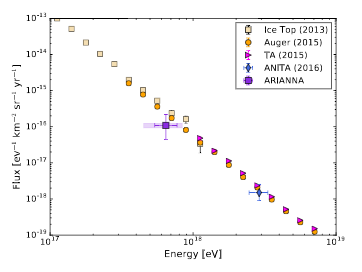
\includegraphics[width=0.6\textwidth]{figures/ARIANNA1.png}
\caption{\label{fig:arianna1} My research on the ARIANNA project has measured cosmic rays with energies of up to $10^{18}$ eV!}
\end{figure}
\end{frame}

\begin{frame}{Voltage, Potential Energy, and Work}
\begin{figure}
\centering
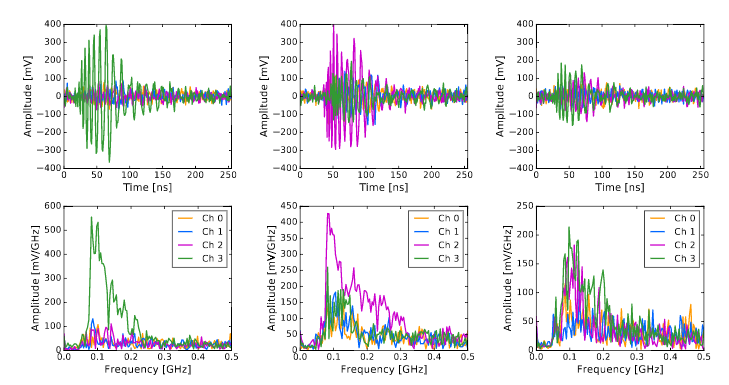
\includegraphics[width=0.6\textwidth]{figures/ARIANNA2.png}
\caption{\label{fig:arianna2} These cosmic rays (protons) have so much energy, that they make radio pulses through the atmosphere.}
\end{figure}
\end{frame}

\begin{frame}{Voltage, Potential Energy, and Work}
\begin{figure}
\centering
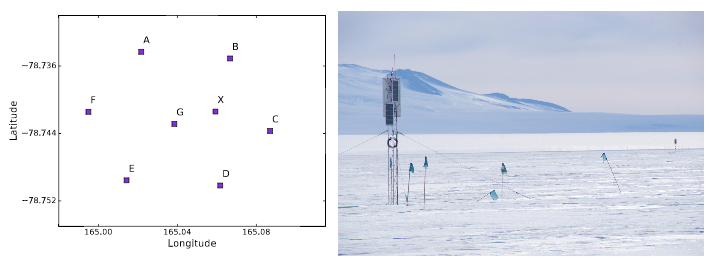
\includegraphics[width=0.6\textwidth]{figures/ARIANNA3.png}
\caption{\label{fig:arianna3} How do we do it?  We build autonomous radio detectors in the Antarctic wilderness... This would make a nice paper topic.}
\end{figure}
\end{frame}

\begin{frame}{Voltage, Potential Energy, and Work}
One electron-Volt is the energy gained by a charge of 1 electron falling through a potential of 1 Volt.
\begin{figure}
\centering
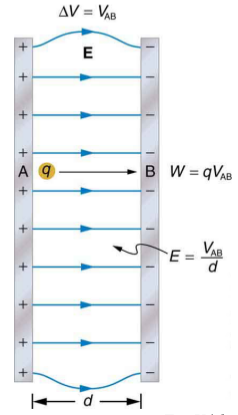
\includegraphics[width=0.25\textwidth]{figures/plates2.png}
\caption{\label{fig:plates2} Fields, voltage, and energy.}
\end{figure}
\end{frame}

\begin{frame}{Voltage, Potential Energy, and Work}
Suppose two objects have the same charge, $-e = -1.6\times 10^{-19}$ C, but one has twice the mass as the other.  If each is released through a potential of 1 V, which object gains more energy?
\begin{itemize}
\item A: The lighter one
\item B: The heavier one
\item C: They gain the same energy
\item D: Cannot determine
\end{itemize}
\end{frame}

\begin{frame}{Voltage, Potential Energy, and Work}
Suppose two objects have the same charge, $-e = -1.6\times 10^{-19}$ C, but one has twice the mass as the other.  If each is released through a potential of 1 V, which object achieves the highest speed?
\begin{itemize}
\item A: The lighter one
\item B: The heavier one
\item C: They gain the same energy
\item D: Cannot determine
\end{itemize}
\end{frame}

\begin{frame}{Voltage, Potential Energy, and Work}
Consider the plates of Fig. \ref{fig:plates2}:
\begin{align}
W &= q\Delta V \\
W &= F\Delta x = qE \Delta x \\
qE \Delta x &= q\Delta V \\
E \Delta x &= \Delta V \\
E &= \frac{\Delta V}{\Delta x}
\end{align}
This derivation is good for a uniform constant field, for example, between two \textit{parallel plates of charge}.  \textbf{We proved that this field is constant back when considering charge distributions.}
\end{frame}

\begin{frame}{Voltage, Potential Energy, and Work}
So what happens if we place an electric field across two parallel plates? A charge +Q on one side and -Q on the other side develops, storing charge.  This is called a \textit{capacitor}.
\begin{figure}
\centering
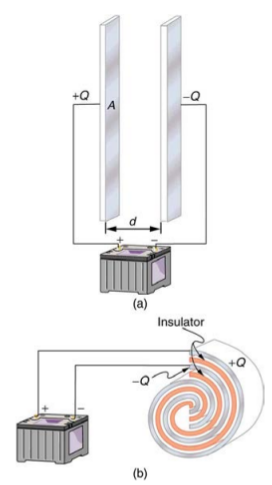
\includegraphics[width=0.25\textwidth]{figures/batt.png}
\caption{\label{fig:batt} A battery is like a parallel plate \textit{capacitor}.}
\end{figure}
\end{frame}

\section{Capacitance}

\begin{frame}{Capacitance}
What voltage is required to store $Q$? Let $\Delta V$ be the voltage difference, $E$ be the electric field strength, and $\Delta x$ be the voltage between the plates.  We already know that
\begin{equation}
\Delta V = E\Delta x
\end{equation}
\textit{But we also know from Coulomb's Law that}
\begin{equation}
E = \frac{\sigma}{\epsilon_0} = \frac{Q}{\epsilon_0 A}
\end{equation}
So we have
\begin{equation}
\Delta V \left(\epsilon_0 \frac{A}{\Delta x}\right) = Q
\end{equation}
So now we know how much charge to expect for a given voltage.
\end{frame}

\begin{frame}{Capacitance}
\begin{equation}
\boxed{
Q = \Delta V \left(\epsilon_0 \frac{A}{\Delta x}\right) = C\Delta V}
\end{equation}
We call the quantity in parentheses the \textit{capacitance} of the capacitor, representing the ability to store charge.  The unit of capacitance is \textbf{the farad}, after Michael Faraday (encounter mid-semester).  Scaling problems in a moment...
\end{frame}

\begin{frame}{Capacitance}
\textbf{Good paper topic:}
\begin{figure}
\centering

\includegraphics[width=0.4\textwidth]{figures/volta.jpg}
\caption{\label{fig:volta2} \small (Lago di Como, Italia) Monument to Alessandro Volta, inventor of the electric battery.}
\end{figure}
\end{frame}

\begin{frame}{Capacitance}
Two batteries store the same charge.  One only needs half the voltage, though.  What is true of the capacitance of the battery with the lower voltage?
\begin{itemize}
\item A: It has half the capacitance
\item B: It has the same capacitance but more charges.
\item C: It has twice the capacitance
\item D: It has half the energy
\end{itemize}
\end{frame}

\begin{frame}{Capacitance}
Two batteries have the same capacitance.  Battery 1 has half the area $A$ as battery 2.  Which of the following is true of battery 2?
\begin{itemize}
\item A: The plates are half the distance ($\Delta x$) apart
\item B: The plates are twice the distance ($\Delta x$) apart
\item C: The plates have half the voltage
\item D: The plates have twice the voltage
\end{itemize}
\end{frame}

\section{More on Point Charges and Voltage}

\begin{frame}{More on Point Charges and Voltage}
We showed in the PhET simulation that the voltage due to a point charge $Q$ is
\begin{equation}
\boxed{
V(r) = \pm k\frac{Q}{r}
}
\end{equation}
Open the PhET again: \url{https://phet.colorado.edu/en/simulation/charges-and-fields}
\begin{itemize}
\item Re-verify that voltage acts like a scalar field: voltage due different point charges just add like numbers
\item \textbf{\alert{Build a battery.  Plot the voltage as a function of distance between the plates.}}
\item (The program only handles 32 separate point charges)
\end{itemize}
\end{frame}

\section{Capacitance and Dielectrics}

\begin{frame}{Capacitance and Dielectrics}
\begin{figure}
\centering
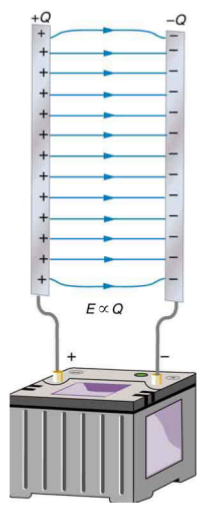
\includegraphics[width=0.25\textwidth]{figures/batt2.png}
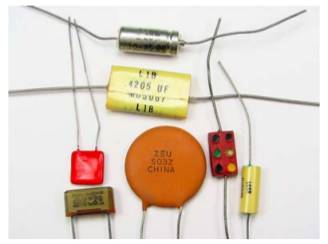
\includegraphics[width=0.5\textwidth]{figures/batt3.png}
\caption{\label{fig:batt2} A battery and a capacitor are not quite the same thing.}
\end{figure}
\end{frame}

\begin{frame}{Capacitance}
Parallel plate capacitor:
\begin{equation}
\boxed{
Q = \Delta V \left(\epsilon_0 \frac{A}{\Delta x}\right) = C\Delta V}
\end{equation}
How can we boost the charge?  Can we increase that $\epsilon_0$?  (It's a small number: $8.85 \times 10^{-12}$ N$^{-1}$ C$^2$ m$^{-2}$).  It turns out that by stuffing some insulating material between the plates \textit{boosts the capacitance...}
\end{frame}

\begin{frame}{Capacitance and Dielectrics}
Because \textit{dielectric} material reduces the field between the plates for the same charge, the voltage corresponding to that charge is reduced.  But that means \textit{higher capacitance}.
\begin{figure}
\centering
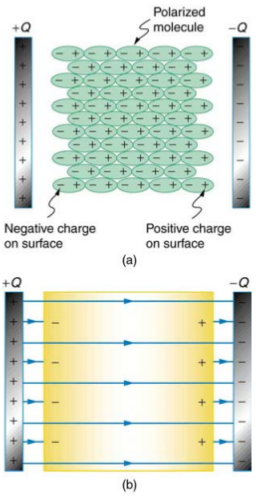
\includegraphics[width=0.25\textwidth]{figures/polar.png}
\caption{\label{fig:polar} Polarized dielectric.}
\end{figure}
\end{frame}

\begin{frame}{Capacitance and Dielectrics}
\begin{figure}
\centering
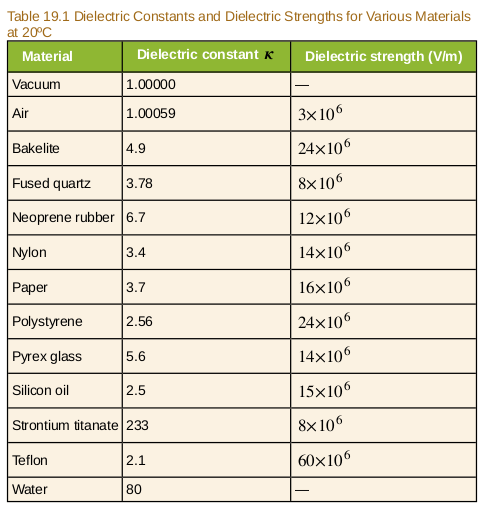
\includegraphics[width=0.5\textwidth]{figures/tableK.png}
\caption{\label{fig:tab} The middle column is the number by which $\epsilon_0$ is scaled up when dielectric is introduced.  We can't play this game indefinitely, because materials have a maximum electric field (third column) they can handle before they're ripped apart.}
\end{figure}
\end{frame}

\begin{frame}{Capacitance and Dielectrics}
\textbf{Group board exercise:} Suppose a capacitor (parallel plate) has area $A = 1$ cm$^2$ and separation $d = 1$ mm.  Using $\epsilon_0 = 8.85 \times 10^{-12}$ C$^2$ N$^{-1}$ m$^{-2}$, calculate the capacitance.  How much charge will be stored if we place 9 V across the capacitor?
\end{frame}

\begin{frame}{Capacitance and Dielectrics}
\textbf{Group board exercise:} Suppose we fill the capacitor with Teflon (see Tab. \ref{fig:tab}).  How much charge can we store with 9 V?
\end{frame}

\begin{frame}{Capacitance and Dielectrics}
\begin{figure}
\centering
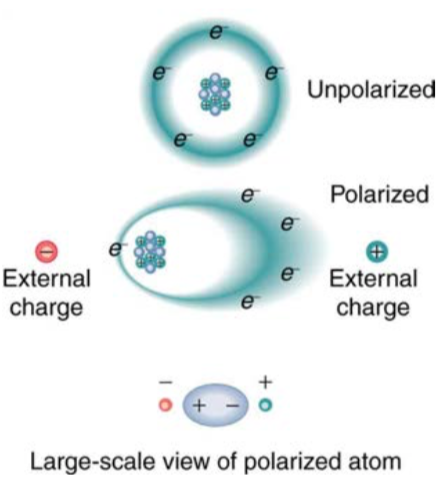
\includegraphics[width=0.5\textwidth]{figures/polar2.png}
\caption{\label{fig:polar2} Taking advantage of atomic structure in the dielectric.}
\end{figure}
\end{frame}

\begin{frame}{Capacitance and Dielectrics}
\begin{figure}
\centering
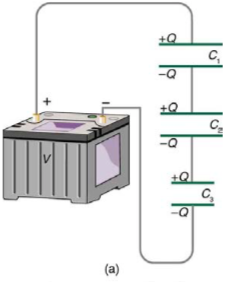
\includegraphics[width=0.4\textwidth]{figures/cap1.png} \hspace{0.2cm}
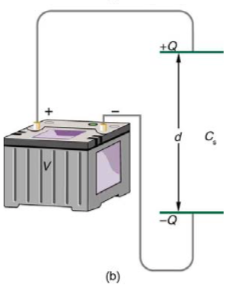
\includegraphics[width=0.4\textwidth]{figures/cap2.png}
\caption{\label{fig:cap} How do we compute the total capacitance of (a) such that we know the charge stored for a given voltage in (b)?}
\end{figure}
\end{frame}

\begin{frame}{Capacitance and Dielectrics}
\begin{itemize}
\item Notice that \textit{charge is conserved}, so $Q$ has to be the same on all capacitors
\item But that means the \textit{voltage} on the different capacitors has to obey
\begin{equation}
V = V_1 + V_2 + V_3
\end{equation}
and
\begin{align}
Q &= C_1 V_1 \\
Q &= C_2 V_2 \\
Q &= C_3 V_3
\end{align}
\end{itemize}
\end{frame}

\begin{frame}{Capacitance and Dielectrics}
\begin{itemize}
\item Combining equations:
\begin{align}
V &= \frac{Q}{C_{\rm total}} = \frac{Q}{C_1}+\frac{Q}{C_2}+\frac{Q}{C_3} \\
\frac{1}{C_{\rm total}} &= \frac{1}{C_1}+\frac{1}{C_2}+\frac{1}{C_3}
\end{align}
\item This is the capacitance for capacitors connected \textbf{in series}.
\end{itemize}
\end{frame}

\begin{frame}{Capacitance and Dielectrics}
\begin{figure}
\centering
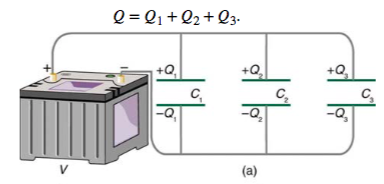
\includegraphics[width=0.4\textwidth]{figures/cap3.png} \hspace{0.2cm}
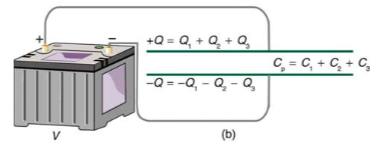
\includegraphics[width=0.4\textwidth]{figures/cap4.png}
\caption{\label{fig:cap2} How do we compute the total capacitance of (a) such that we know the charge stored for a given voltage in (b)?}
\end{figure}
\end{frame}

\begin{frame}{Capacitance and Dielectrics}
The result is:
\begin{equation}
C_{\rm total} = C_1+C_2+C_3
\end{equation}
This is the capacitance for capacitors connected \textbf{in parallel}.
\end{frame}

\begin{frame}{Capacitance and Dielectrics}
Suppose a circuit has two identical capacitors connected \textbf{in parallel}.  If a voltage of 9V stores $9 \times 10^{-6}$ C or $9\mu$C of charge, how much charge would be stored if we add two more of these same capacitors in parallel to the circuit?
\begin{itemize}
\item A: 9 $\mu$C
\item B: 4.5 $\mu$C
\item C: 18 $\mu$C
\item D: 32 $\mu$C
\end{itemize}
\end{frame}

\begin{frame}{Capacitance and Dielectrics}
Suppose we have a circuit where two capacitors are connected \textbf{in series}, and each has a \textit{capacitance} of $2\mu$F (a microfarad).  What is the total capacitance?
\begin{itemize}
\item A: $1\mu$F
\item B: $2\mu$F
\item C: $4\mu$F
\item D: $8\mu$F
\end{itemize}
\end{frame}

\begin{frame}{Capacitance and Dielectrics}
Why is the capacitance reduced by adding another capacitor?  What physically is occurring to reduce capacitance?
\begin{itemize}
\item A: It's as if the cross-sectional area is being decreased.
\item B: It's as if the plate separation is being increased.
\item C: It's as if the dielectric constant is being reduced.
\item D: It's as if the plate separation is being decreased.
\end{itemize}
\end{frame}

\section{Conclusion}

\begin{frame}{Unit 1 Summary}
\textbf{Reading: Chapters 18 and 19}
\begin{enumerate}
\item Charge, mass, the Coulomb force, and the gravitational force
\item Force fields
\item Electric potential and capacitance
\end{enumerate}
\end{frame}

\section{Answers}

\begin{frame}{Answers}
\tiny
\begin{columns}[T]
\begin{column}{0.5\textwidth}
\begin{itemize}
\item It is zero.
\item Entropy has increased, but the internal energy returns to the original value
\item 0.5
\item The system does work equal to 0.5 liters times 1 atm
\item +1
\item The negative charges in the conductor move toward the positive charges in the rod.
\item B and C
\item The charges accelerate towards each other.
\item The charges $-2q$ accelerate towards the charge $+q$.
\item They are probably $\vec{v}_{\rm i} = -\hat{i}-\hat{j}$
\item They are probably $\vec{v}_{\rm i} = \hat{i}-\hat{j}$
\item 45 deg
\item Symmetry
\item About 25 deg (26.56 degrees)
\item Taking the value $z = R$ represents a minimum in the field strength.
\item The field is constant.
\item $\frac{\sigma}{\epsilon_0}$ N/C
\item 0 N/C
\end{itemize}
\end{column}
\begin{column}{0.5\textwidth}
\begin{itemize}
\item The total charge on the ring
\item A point charge $Q_{\rm tot}$
\item $mgh$
\item $-mg$
\item $W = \vec{F} \cdot \vec{x} = Fx\cos\theta$
\item 60 kJ and 720 kJ, respectively
\item About 7 hours
\item About 10 kJ
\item About 6 minutes
\item 9 V
\item 20 kJ
\item 36 hours
\item They gain the same energy
\item The lighter one
\item It has twice the capacitance
\item The plates are half the distance ($\Delta x$) apart
\item 18 $\mu$C
\item $1\mu$F
\item It's as if the plate separation is being increased.
\end{itemize}
\end{column}
\end{columns}
\end{frame}

\end{document}
